% !TEX program = pdflatex
% Standalone, all-English LaTeX source.
% Compile with pdfLaTeX, XeLaTeX, or LuaLaTeX.
% No external bibliography, image, CSV, or project files are required.
% Original data snapshot: October 3, 2026.
% English archive edition prepared on October 5, 2026.
\documentclass[11pt,a4paper]{article}
\usepackage[T1]{fontenc}
\usepackage{lmodern}
\usepackage[english]{babel}
\usepackage{geometry}
\geometry{left=24mm,right=24mm,top=23mm,bottom=23mm}
\usepackage{amsmath,amssymb,bm}
\usepackage{booktabs,array,tabularx,longtable}
\usepackage{xcolor,graphicx}
\usepackage{tikz}
\usetikzlibrary{arrows.meta,positioning}
\usepackage{listings}
\usepackage{xurl}
\usepackage[unicode,hidelinks]{hyperref}

\hypersetup{
  pdftitle={A Football Video Analysis Prototype: From Object Detection to Local Trajectory Statistics},
  pdfauthor={JIAHE35},
  pdfsubject={Soccer-Video-Analysis V0.1--V0.7 Project Completion Report}
}
\linespread{1.12}
\setlength{\parindent}{1.2em}
\setlength{\parskip}{0.25em}
\renewcommand{\arraystretch}{1.16}
\setlength{\tabcolsep}{5pt}
\setlength{\emergencystretch}{2em}
\newcolumntype{L}{>{\raggedright\arraybackslash}X}
\newcommand{\code}[1]{\texttt{\detokenize{#1}}}
\newcommand{\ROI}{\mathcal{R}}
\newcommand{\HeatMax}{2.566667}
\definecolor{heatLow}{RGB}{35,80,160}
\definecolor{heatMid}{RGB}{246,217,74}
\definecolor{heatHigh}{RGB}{217,63,49}
\definecolor{pitchPaper}{RGB}{244,247,244}
\definecolor{roiPaper}{RGB}{225,237,226}
\definecolor{observedBlue}{RGB}{45,102,166}
\definecolor{predictedGold}{RGB}{238,190,62}
\lstset{
  basicstyle=\ttfamily\footnotesize,
  columns=fullflexible,
  breaklines=true,
  keepspaces=true,
  showstringspaces=false,
  frame=single,
  rulecolor=\color{black!20},
  xleftmargin=0.5em,
  xrightmargin=0.5em,
  aboveskip=0.8em,
  belowskip=0.8em
}

% Heat values are cumulative accepted person-seconds in nominal 1 m cells.
% Both panels use the same maximum. This palette is for the paper, not a
% byte-for-byte reproduction of the OpenCV PNG's color map.
\newcommand{\HeatCell}[3]{%
  \pgfmathtruncatemacro{\heatpct}{min(100,round(100*#3/\HeatMax))}%
  \ifnum\heatpct<50
    \pgfmathtruncatemacro{\heatblend}{2*\heatpct}%
    \colorlet{heatcell}{heatMid!\heatblend!heatLow}%
  \else
    \pgfmathtruncatemacro{\heatblend}{2*\heatpct-100}%
    \colorlet{heatcell}{heatHigh!\heatblend!heatMid}%
  \fi
  \fill[heatcell] (#1,#2) rectangle ({#1+1},{#2+1});%
}

% BEGIN GENERATED HEAT DATA
\newcommand{\TeamAHeatCells}{
\HeatCell{88}{42}{0.166667}
\HeatCell{88}{43}{0.033333}
\HeatCell{89}{21}{0.166667}
\HeatCell{89}{22}{0.066667}
\HeatCell{89}{42}{0.433333}
\HeatCell{90}{20}{0.100000}
\HeatCell{90}{21}{0.100000}
\HeatCell{90}{36}{0.566667}
\HeatCell{90}{41}{0.333333}
\HeatCell{91}{18}{0.066667}
\HeatCell{91}{19}{0.100000}
\HeatCell{91}{20}{0.100000}
\HeatCell{91}{35}{1.000000}
\HeatCell{91}{36}{0.966667}
\HeatCell{91}{37}{0.133333}
\HeatCell{91}{40}{0.033333}
\HeatCell{91}{41}{0.233333}
\HeatCell{92}{16}{0.200000}
\HeatCell{92}{17}{0.300000}
\HeatCell{92}{18}{0.100000}
\HeatCell{92}{35}{0.366667}
\HeatCell{92}{36}{0.500000}
\HeatCell{92}{37}{0.333333}
\HeatCell{92}{38}{0.233333}
\HeatCell{92}{40}{0.333333}
\HeatCell{93}{14}{0.066667}
\HeatCell{93}{15}{0.266667}
\HeatCell{93}{16}{0.066667}
\HeatCell{93}{29}{0.633333}
\HeatCell{93}{30}{1.000000}
\HeatCell{93}{32}{0.100000}
\HeatCell{93}{34}{0.033333}
\HeatCell{93}{38}{0.066667}
\HeatCell{93}{39}{0.300000}
\HeatCell{93}{40}{0.200000}
\HeatCell{94}{25}{0.033333}
\HeatCell{94}{29}{0.366667}
\HeatCell{94}{30}{1.366667}
\HeatCell{94}{31}{0.366667}
\HeatCell{94}{32}{1.333333}
\HeatCell{94}{33}{0.133333}
\HeatCell{94}{34}{0.033333}
\HeatCell{94}{35}{0.133333}
\HeatCell{95}{29}{0.100000}
\HeatCell{95}{30}{0.166667}
\HeatCell{95}{31}{0.133333}
\HeatCell{95}{32}{0.266667}
\HeatCell{95}{33}{0.933333}
\HeatCell{95}{34}{0.733333}
\HeatCell{96}{29}{0.333333}
\HeatCell{96}{30}{0.933333}
\HeatCell{96}{31}{0.300000}
\HeatCell{96}{32}{0.333333}
\HeatCell{96}{33}{2.566667}
\HeatCell{96}{34}{0.133333}
\HeatCell{97}{28}{0.233333}
\HeatCell{97}{29}{0.533333}
\HeatCell{97}{30}{0.333333}
\HeatCell{97}{31}{0.066667}
\HeatCell{97}{32}{0.700000}
\HeatCell{97}{33}{0.400000}
\HeatCell{97}{34}{0.366667}
\HeatCell{97}{35}{0.300000}
\HeatCell{97}{36}{0.266667}
\HeatCell{97}{37}{0.266667}
\HeatCell{98}{31}{0.133333}
\HeatCell{98}{33}{0.133333}
\HeatCell{98}{34}{2.300000}
\HeatCell{98}{35}{1.600000}
\HeatCell{98}{36}{0.266667}
\HeatCell{98}{37}{0.233333}
\HeatCell{98}{38}{0.133333}
\HeatCell{98}{39}{0.200000}
\HeatCell{98}{40}{0.066667}
\HeatCell{99}{29}{0.133333}
\HeatCell{99}{31}{0.100000}
\HeatCell{99}{34}{0.066667}
\HeatCell{99}{35}{0.333333}
\HeatCell{99}{36}{0.066667}
\HeatCell{99}{37}{0.100000}
\HeatCell{99}{38}{0.166667}
\HeatCell{99}{39}{0.133333}
\HeatCell{99}{40}{0.133333}
\HeatCell{100}{27}{0.033333}
\HeatCell{100}{28}{0.100000}
\HeatCell{100}{29}{0.066667}
\HeatCell{100}{30}{0.033333}
\HeatCell{100}{31}{0.066667}
\HeatCell{100}{32}{0.333333}
\HeatCell{100}{33}{0.066667}
\HeatCell{100}{34}{0.133333}
\HeatCell{100}{35}{0.200000}
\HeatCell{100}{36}{0.100000}
\HeatCell{100}{39}{0.200000}
\HeatCell{100}{40}{0.166667}
\HeatCell{100}{41}{0.133333}
\HeatCell{100}{42}{0.133333}
\HeatCell{101}{25}{0.100000}
\HeatCell{101}{26}{0.133333}
\HeatCell{101}{28}{0.066667}
\HeatCell{101}{30}{0.066667}
\HeatCell{101}{31}{0.166667}
\HeatCell{101}{33}{0.033333}
\HeatCell{102}{24}{0.033333}
\HeatCell{102}{34}{0.300000}
\HeatCell{102}{35}{0.066667}
\HeatCell{103}{27}{0.033333}
\HeatCell{103}{34}{1.033333}
\HeatCell{103}{35}{0.200000}
\HeatCell{104}{26}{0.133333}
\HeatCell{104}{27}{0.066667}
}

\newcommand{\TeamBHeatCells}{
\HeatCell{88}{30}{0.166667}
\HeatCell{88}{31}{0.633333}
\HeatCell{88}{46}{0.200000}
\HeatCell{89}{28}{0.033333}
\HeatCell{89}{29}{0.066667}
\HeatCell{89}{30}{0.433333}
\HeatCell{89}{31}{1.333333}
\HeatCell{89}{45}{0.266667}
\HeatCell{89}{46}{0.233333}
\HeatCell{90}{25}{0.166667}
\HeatCell{90}{26}{0.166667}
\HeatCell{90}{27}{0.600000}
\HeatCell{90}{28}{0.500000}
\HeatCell{90}{37}{0.133333}
\HeatCell{90}{44}{0.266667}
\HeatCell{90}{45}{0.233333}
\HeatCell{91}{22}{0.200000}
\HeatCell{91}{23}{0.100000}
\HeatCell{91}{24}{0.300000}
\HeatCell{91}{25}{0.133333}
\HeatCell{91}{28}{0.266667}
\HeatCell{91}{37}{0.166667}
\HeatCell{91}{43}{0.300000}
\HeatCell{91}{44}{0.066667}
\HeatCell{92}{16}{0.133333}
\HeatCell{92}{17}{0.066667}
\HeatCell{92}{19}{0.133333}
\HeatCell{92}{20}{0.166667}
\HeatCell{92}{21}{0.333333}
\HeatCell{92}{22}{0.033333}
\HeatCell{92}{27}{0.333333}
\HeatCell{92}{37}{0.066667}
\HeatCell{92}{38}{0.200000}
\HeatCell{92}{42}{0.700000}
\HeatCell{92}{43}{0.133333}
\HeatCell{93}{17}{0.466667}
\HeatCell{93}{18}{0.266667}
\HeatCell{93}{19}{0.033333}
\HeatCell{93}{25}{0.233333}
\HeatCell{93}{26}{1.100000}
\HeatCell{93}{27}{0.200000}
\HeatCell{93}{35}{0.066667}
\HeatCell{93}{38}{0.200000}
\HeatCell{93}{39}{0.033333}
\HeatCell{93}{41}{0.100000}
\HeatCell{93}{42}{1.966667}
\HeatCell{93}{43}{0.233333}
\HeatCell{94}{16}{0.033333}
\HeatCell{94}{17}{0.066667}
\HeatCell{94}{24}{0.300000}
\HeatCell{94}{25}{0.666667}
\HeatCell{94}{35}{0.033333}
\HeatCell{94}{38}{0.100000}
\HeatCell{94}{39}{0.100000}
\HeatCell{94}{41}{0.800000}
\HeatCell{94}{42}{1.266667}
\HeatCell{95}{24}{0.533333}
\HeatCell{95}{31}{0.333333}
\HeatCell{95}{35}{0.100000}
\HeatCell{95}{36}{0.066667}
\HeatCell{95}{38}{0.100000}
\HeatCell{95}{39}{0.166667}
\HeatCell{96}{23}{0.466667}
\HeatCell{96}{24}{0.033333}
\HeatCell{96}{29}{0.066667}
\HeatCell{96}{30}{2.400000}
\HeatCell{96}{31}{0.466667}
\HeatCell{96}{32}{0.033333}
\HeatCell{96}{36}{0.033333}
\HeatCell{96}{38}{0.100000}
\HeatCell{96}{39}{0.100000}
\HeatCell{97}{22}{0.066667}
\HeatCell{97}{23}{0.166667}
\HeatCell{97}{28}{0.100000}
\HeatCell{97}{29}{0.533333}
\HeatCell{97}{30}{0.433333}
\HeatCell{97}{31}{0.100000}
\HeatCell{97}{33}{0.066667}
\HeatCell{97}{36}{0.033333}
\HeatCell{97}{38}{0.266667}
\HeatCell{98}{22}{0.400000}
\HeatCell{98}{27}{0.066667}
\HeatCell{98}{28}{1.033333}
\HeatCell{98}{29}{0.600000}
\HeatCell{98}{30}{1.133333}
\HeatCell{98}{31}{0.933333}
\HeatCell{98}{32}{0.533333}
\HeatCell{98}{33}{0.966667}
\HeatCell{98}{38}{0.366667}
\HeatCell{99}{21}{0.166667}
\HeatCell{99}{25}{0.033333}
\HeatCell{99}{26}{0.200000}
\HeatCell{99}{27}{0.133333}
\HeatCell{99}{28}{0.966667}
\HeatCell{99}{29}{0.600000}
\HeatCell{99}{30}{1.000000}
\HeatCell{99}{31}{1.333333}
\HeatCell{99}{32}{1.200000}
\HeatCell{99}{33}{0.900000}
\HeatCell{99}{36}{0.100000}
\HeatCell{99}{37}{2.000000}
\HeatCell{99}{38}{0.166667}
\HeatCell{100}{21}{0.233333}
\HeatCell{100}{25}{0.033333}
\HeatCell{100}{27}{0.200000}
\HeatCell{100}{28}{0.266667}
\HeatCell{100}{30}{0.066667}
\HeatCell{100}{31}{0.066667}
\HeatCell{100}{32}{2.233333}
\HeatCell{100}{33}{0.666667}
\HeatCell{100}{36}{0.500000}
\HeatCell{100}{37}{0.266667}
\HeatCell{100}{38}{0.433333}
\HeatCell{100}{39}{0.066667}
\HeatCell{101}{21}{0.166667}
\HeatCell{101}{25}{0.100000}
\HeatCell{101}{26}{0.066667}
\HeatCell{101}{29}{0.033333}
\HeatCell{101}{32}{0.666667}
\HeatCell{101}{33}{0.200000}
\HeatCell{101}{35}{0.033333}
\HeatCell{101}{36}{0.466667}
\HeatCell{101}{38}{1.633333}
\HeatCell{101}{39}{0.066667}
\HeatCell{102}{25}{0.033333}
\HeatCell{102}{33}{0.333333}
\HeatCell{102}{34}{0.500000}
\HeatCell{102}{35}{0.433333}
\HeatCell{102}{36}{0.100000}
\HeatCell{102}{38}{1.766667}
\HeatCell{103}{21}{0.066667}
\HeatCell{103}{32}{0.100000}
\HeatCell{103}{33}{2.333333}
\HeatCell{103}{34}{0.200000}
\HeatCell{103}{35}{0.066667}
\HeatCell{103}{36}{0.033333}
\HeatCell{104}{30}{0.033333}
\HeatCell{104}{31}{0.100000}
\HeatCell{104}{32}{0.166667}
\HeatCell{104}{33}{0.433333}
\HeatCell{104}{35}{0.166667}
\HeatCell{104}{36}{1.066667}
}

% END GENERATED HEAT DATA

\newcommand{\PitchHeatPanel}[2]{%
  \begin{tikzpicture}[x=0.085cm,y=-0.085cm]
    \fill[pitchPaper] (52.5,0) rectangle (105,68);
    \fill[roiPaper] (88.5,13.84) rectangle (105,54.16);
    \begin{scope}
      \clip (88.5,13.84) rectangle (105,54.16);
      #2
    \end{scope}
    \draw[black!60,line width=0.45pt] (52.5,0) rectangle (105,68);
    \draw[black!60,line width=0.45pt]
      (105,13.84)--(88.5,13.84)--(88.5,54.16)--(105,54.16);
    \draw[black!60,line width=0.45pt]
      (105,24.84)--(99.5,24.84)--(99.5,43.16)--(105,43.16);
    \draw[black!60,line width=0.45pt]
      (105,30.34)--(107,30.34)--(107,37.66)--(105,37.66);
    \draw[black!60,line width=0.45pt,domain=126.95:233.05,samples=45]
      plot ({94+9.15*cos(\x)},{34+9.15*sin(\x)});
    \draw[black!60,line width=0.45pt,domain=-90:90,samples=45]
      plot ({52.5+9.15*cos(\x)},{34+9.15*sin(\x)});
    \fill[black!60] (94,34) circle[radius=0.35];
    \node[anchor=south west,font=\small\bfseries] at (52.5,-2) {#1};
  \end{tikzpicture}%
}

\title{\textbf{A Football Video Analysis Prototype:\\
From Object Detection to Local Trajectory Statistics}\\[0.5em]
\large An Iterative Engineering Study of YOLO11 and ByteTrack, V0.1--V0.7}
\author{JIAHE35\\
  \small Independent Project: Soccer-Video-Analysis\\
  \small \url{https://github.com/JIAHE35/Soccer-Video-Analysis}}
\date{October 5, 2026\\
  \small English Archive Edition; Data Snapshot: October 3, 2026}

\begin{document}
\maketitle

\begin{abstract}
This report documents the development of an independent football-video analysis
prototype, from basic object detection to restricted spatial statistics.
A pretrained YOLO11n detector is combined with grass-neighborhood filtering
to reduce off-field person annotations, ByteTrack for temporary person IDs,
and match-specific kit-color classification with temporal voting for teams,
goalkeepers, referees, and unknown roles. The ball is handled by an independent
detection and short-term association branch, without person-style IDs; model
detections and missing-frame predictions are recorded separately.
Because the input is a highlight video captured by a moving broadcast camera,
the project does not apply one fixed homography to the entire video. Instead,
a continuous 11.9-second shot is calibrated at 13 manual keyframes, with mapping
restricted to the right penalty area. The final outputs are short 2D trajectories,
two-team position heatmaps, and a data-quality report. The selected shot contains
357 frames and 4,281 object records, of which 2,904 fall inside the valid mapping
region. Ball detections, predictions, and missing outputs cover 146, 78, and
133 frames, respectively. Eighty automated tests passed during the original
snapshot verification. These findings demonstrate an operational, traceable
engineering pipeline, not validated detection accuracy, physical motion
estimates, possession statistics, or full-match tactical analysis. The principal
value of the project is its incremental implementation, explicit data semantics,
restricted scope, and documented limitations.
\end{abstract}

\noindent\textbf{Keywords:} football video analysis; YOLO11; ByteTrack;
homography; short-term trajectories; position heatmaps; reproducible engineering;
data quality

\tableofcontents
\clearpage

\section{Introduction}

Football videos contain players, referees, goalkeepers, the ball, spectators,
advertising boards, and other visual objects. For an independent learning
project, attempting to build a complete match-analysis system immediately
introduces detection, tracking, identity, camera geometry, and statistical
interpretation problems at the same time. This makes the source of an error
difficult to isolate. The project therefore follows an incremental strategy:
first establish the smallest complete video-input, detection, annotation,
and video-output workflow, then add modules in response to observed failures.

The initial objective was to run a football video through a pretrained detector
and produce a video with bounding boxes. Subsequent versions addressed
spectator annotations, person IDs, team and role classification, intermittent
ball detections, local 2D mapping, and trajectory and position-distribution
visualizations. A separate document is retained for each version so that the
latest README does not erase earlier design decisions or experimental boundaries.

This is an engineering completion report, not a proposal for a new detection
network or tracking algorithm. Its main contributions are:
\begin{enumerate}
  \item an operational pipeline from video to structured object records and
        restricted 2D analysis;
  \item explicit separation of temporary person IDs, observed ball detections,
        predicted ball positions, and invalid mappings;
  \item geometric scope restrictions appropriate to highlight footage and
        moving-camera conditions;
  \item a record of the V0.1--V0.7 development process, automated verification,
        and remaining failure risks.
\end{enumerate}

\section{Technical Background and Problem Definition}

\subsection{Pretrained Detection and Tracking}

The project uses YOLO11n weights provided by Ultralytics without
football-specific training or fine-tuning. The official documentation describes
the model's detection interface and pretrained usage\cite{yolo11}.
The general-purpose \code{person} class does not distinguish players, referees,
goalkeepers, and spectators. Football roles are therefore assigned by downstream
heuristics, not by native fine-grained football categories in the detector.

ByteTrack associates detection boxes over time and uses lower-confidence
detections as additional association evidence\cite{bytetrack}.
The project calls an existing implementation rather than reimplementing the
core algorithm. A track ID represents a temporary temporal association:
it is neither a jersey number nor a verified real-player identity.

\subsection{Restricted Planar Mapping}

A homography describes a projective relationship between planes and can relate
approximately coplanar pitch reference points to image positions\cite{opencv}.
The particular keyframe annotations, valid region, and interpolation rules used
here are engineering choices for this project, not a general automatic
camera-calibration solution.

The pipeline addresses three distinct questions:
\begin{enumerate}
  \item \textbf{Detection:} which image regions may contain an object in the
        current frame?
  \item \textbf{Association:} do records in adjacent frames belong to the same
        temporary track?
  \item \textbf{Statistics:} how should position samples be aggregated when
        geometry and identity evidence permit?
\end{enumerate}
A downstream visualization does not automatically correct errors introduced
by an earlier stage.

\section{Data, Environment, and Experimental Scope}

\subsection{Input Footage}

The project user supplied an approximately two-minute football highlight video.
Its match provenance, capture parameters, and permission for redistribution
have not been independently verified. It is not presented as a public benchmark
dataset. The normalized input is \path{data/soccervideo_cfr.mp4}, with a resolution
of $1280\times588$, a frame rate of 30 FPS, 3,534 frames, and a duration of
117.8 seconds.

Early inspection identified variable-frame-rate input. Writing such input at
an average frame rate can produce inconsistent playback timing. The project
therefore converts a copy to constant 30 FPS while preserving the original
footage. FFmpeg frame-rate and trimming filters provide timeline normalization
and continuous-shot extraction\cite{ffmpeg}. Normalization supports frame
alignment but does not remove compression artifacts or recover missing
visual detail.

\subsection{Local Research Clip}

V0.6 and V0.7 use the following interval on the source-file timeline:
\[
  74.7 \leq t < 86.6\ \mathrm{s}.
\]
This corresponds to zero-based source frames 2241--2597: 357 frames and
11.9 seconds. These times are not the broadcast match-clock readings.
The independent clip is saved as \path{data/v06_homography_clip.mp4}.

The clip is a continuous shot, but the camera pans and zooms.
The valid analysis region is restricted to the right penalty area and does not
cover the entire pitch. Pitch dimensions are nominally assumed to be
$105\times68$ meters; no stadium survey was performed.

\subsection{Environment Snapshot and Unmeasured Metrics}

Table~\ref{tab:env} records the local software versions read during preparation
of the original report. It does not imply that every historical version used
exactly the same environment. The requirements file does not pin all dependency
versions, so rerunning the project in another environment may produce different
records.

\begin{table}[htbp]
\centering
\caption{Local software environment snapshot.}
\label{tab:env}
\begin{tabular}{ll}
\toprule
Component & Version or description\\
\midrule
Operating-system interface & Darwin / macOS\\
Python & 3.12.0\\
Ultralytics & 8.4.155\\
OpenCV Python & 5.0.0.93\\
NumPy & 2.5.3\\
LAP & 0.5.13\\
Detection weights & \code{yolo11n.pt}\\
Training strategy & No custom training or fine-tuning\\
\bottomrule
\end{tabular}
\end{table}

The project has no complete manually annotated dataset and no standardized
hardware inference-time measurements for comparison. This report does not
provide precision, recall, mAP, IDF1, HOTA, or real-time processing speed.
Official model metrics measured on other datasets cannot substitute for an
evaluation of this project.

\section{Version Evolution and Overall Architecture}

\begin{table}[htbp]
\centering
\caption{Development milestones from V0.1 to V0.7.}
\label{tab:versions}
\small
\begin{tabularx}{\linewidth}{@{}lLL@{}}
\toprule
Version & Added capability & Motivation\\
\midrule
V0.1 & Pretrained detection, colored boxes, and video output
     & Verify the minimal end-to-end workflow\\
V0.2 & Grass support and class-specific thresholds
     & Reduce annotations in stands and off-field regions\\
V0.3 & ByteTrack person IDs and independent ball detection
     & Establish short-term person association and retain small-ball candidates\\
V0.4 & Kit colors, goalkeeper configuration, role voting, and CSV export
     & Distinguish teams and roles and preserve structured results\\
V0.5 & Single-ball association, short-gap prediction, and explicit states
     & Address intermittent ball detection and some pitch-mark false positives\\
V0.6 & Manual keyframe homographies and restricted pitch mapping
     & Enable a local 2D view under moving-camera conditions\\
V0.7 & Short trajectories, team position heatmaps, and quality summaries
     & Aggregate existing coordinates and expose continuity problems\\
\bottomrule
\end{tabularx}
\end{table}

V0.1 used a shared confidence threshold of 0.25. The final V0.2 settings were
0.5 for people and 0.3 for the ball; from V0.3 onward, the ball candidate
threshold was lowered to 0.18. The V0.2--V0.3 video comparison therefore changes
both tracking and the ball threshold. It is not a single-factor tracking
ablation. The current detection entry point retains the V0.5 detection logic,
while V0.6 and V0.7 add downstream functionality by reading existing CSV files.

\begin{figure}[htbp]
\centering
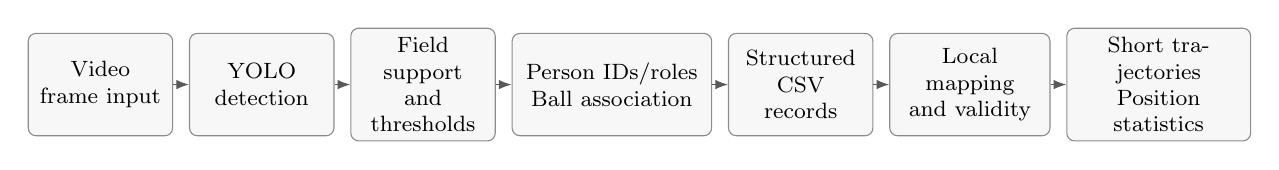
\begin{tikzpicture}[
  box/.style={draw=black!45,fill=black!3,rounded corners=1mm,
    minimum height=13mm,text width=16mm,align=center,font=\footnotesize},
  flow/.style={-{Latex[length=1.6mm]},draw=black!65}
]
\node[box] (v) {Video\\frame input};
\node[box,right=2mm of v] (d) {YOLO\\detection};
\node[box,right=2mm of d] (f) {Field support\\and thresholds};
\node[box,right=2mm of f,text width=23mm] (r) {Person IDs/roles\\Ball association};
\node[box,right=2mm of r] (c) {Structured\\CSV records};
\node[box,right=2mm of c,text width=18mm] (h) {Local mapping\\and validity};
\node[box,right=2mm of h,text width=21mm] (a) {Short trajectories\\Position statistics};
\draw[flow] (v)--(d);
\draw[flow] (d)--(f);
\draw[flow] (f)--(r);
\draw[flow] (r)--(c);
\draw[flow] (c)--(h);
\draw[flow] (h)--(a);
\end{tikzpicture}
\caption{Logical workflow. Person and ball association use separate branches.
V0.6 and V0.7 reuse existing records without rerunning detection.}
\end{figure}

\section{Methods}

\subsection{Class-Specific Detection Thresholds and Field Support}

The current person display threshold is 0.5, while person detections down to
0.1 are passed to the ByteTrack pipeline. Ball detection uses a separate
inference branch with a candidate threshold of 0.18. This separates person
display requirements from the need to retain small-ball candidates.
A confidence score is a model output, not a probability of a true object
calibrated by this project.

An HSV grass mask is constructed for each frame. For a bounding box
$b=(x_1,y_1,x_2,y_2)$, the anchor is defined as
\begin{equation}
 \mathbf{a}(b)=
 \begin{cases}
 ((x_1+x_2)/2,\ y_2), & \text{person};\\
 ((x_1+x_2)/2,\ (y_1+y_2)/2), & \text{ball}.
 \end{cases}
\end{equation}
A grass-pixel ratio of at least 0.25 in the anchor neighborhood provides
field support. For close-up people cropped at the bottom of the frame, an
additional lower-box-region check is used. This is a color heuristic rather
than semantic pitch segmentation. It can still fail near advertising boards
or when lighting changes the grass mask.

\subsection{Person IDs and Match-Specific Roles}

ByteTrack establishes short-term person associations; the ball does not enter
the person-ID branch. Before annotations are drawn, role classification
extracts a central upper-body crop: approximately 20\%--80\% of the box width
and 12\%--55\% of the box height. Match-specific HSV masks produce role candidates,
and per-ID temporal voting reduces single-frame label flicker.

The current defaults map red kits to Team A, white kits to Team B, black kits
to referees, and blue kits to the Team B goalkeeper. The Team A goalkeeper's
kit has not been established, so that configuration is disabled by default.
The project cannot claim reliable identification of both teams' goalkeepers.
Ambiguous, undersized, or unconfigured appearances remain \code{unknown}.

This classifier does not read names or jersey numbers and is not a trained
referee classifier. Staff wearing similar colors can be misclassified.
ID switches may transfer or disrupt role history. YOLO confidence in the CSV
describes the detection box; it must not be interpreted as confidence in the
assigned team or referee role.

\subsection{Independent Ball Association and Short-Gap Prediction}

V0.5 adds shape, appearance, and temporal-association checks after ball
candidate thresholding. The maximum candidate side length is 48 pixels,
and the width-to-height ratio must lie between 0.35 and 1.8.
Appearance evidence uses grayscale standard deviation or color saturation,
with default thresholds of 25 and 180, respectively, to suppress some smooth
white pitch markings.

A tentative track requires at least two nearby detections for confirmation.
A low-confidence initial track also requires evidence such as proximity to
a player, clear displacement, or sufficiently high historical confidence,
rather than confirmation solely from a persistent stationary white point.
A confirmed track selects candidates near its predicted position and produces
at most one ball result per frame.

Let successive accepted detections be separated by $\Delta$ frames, and let
$\mathbf{c}_t$ be the detected center. The observed and smoothed image velocities
are
\begin{align}
 \mathbf{v}^{\mathrm{obs}}_t
   &=\frac{\mathbf{c}_t-\mathbf{c}_{t-\Delta}}{\Delta},\\
 \widehat{\mathbf{v}}_t
   &=\lambda\widehat{\mathbf{v}}_{\mathrm{prev}}
     +(1-\lambda)\mathbf{v}^{\mathrm{obs}}_t,
 \qquad \lambda=0.65.
\end{align}
During missing detections, constant-velocity extrapolation in image coordinates
uses $\widehat{\mathbf{c}}_{t+1}
=\widehat{\mathbf{c}}_t+\widehat{\mathbf{v}}$.
Predictions last for at most eight consecutive frames, approximately
0.27 seconds at 30 FPS. The base association distance is 120 pixels, with a
moderately expanded search region as missing frames accumulate.

The CSV distinguishes \code{detected} from \code{predicted}.
Predictions use dashed boxes and have no YOLO detection confidence.
A prediction is an estimate, not a new model detection. Abrupt stops, kicks,
occlusion, and camera motion can invalidate the constant-velocity assumption.

\subsection{Manual Keyframe Homographies}

The relationship between an image point $(u,v)$ and a nominal pitch point
$(x,y)$ is
\begin{equation}
 s
 \begin{bmatrix}x\\y\\1\end{bmatrix}
 =
 \mathbf{H}_t
 \begin{bmatrix}u\\v\\1\end{bmatrix}.
\end{equation}
The coordinate convention places the right goal at $x=105$ and the far
touchline at $y=0$. The valid region is
\begin{equation}
 \ROI=[88.5,105]\times[13.84,54.16].
\end{equation}
Each keyframe uses at least four named, non-collinear, visible ground-plane
references. These include penalty-area or goal-area corners, penalty-arc
intersections, the penalty spot, the far pitch corner, and goalpost bases.
Goalpost tops are not ground-plane points and are excluded.

The local keyframes are
$0,30,60,90,120,150,180,210,240,270,300,330,356$.
Occluded goal-area corners are not forced into the annotation.
The far goal-area corner is omitted at frames 90, 270, 300, and 330.

\subsection{Restricted Interpolation for Camera Motion}

Homography coefficients are not interpolated directly.
For neighboring keyframes indexed by $k$ and $k+1$, the four valid-region
corners $\mathbf{q}_j$ are inverse-projected into both images, producing
$\mathbf{p}_{k,j}$ and $\mathbf{p}_{k+1,j}$.
For an intermediate frame $t$,
\begin{align}
 \alpha &=\frac{t-f_k}{f_{k+1}-f_k},\\
 \mathbf{p}_{t,j}
   &=(1-\alpha)\mathbf{p}_{k,j}+\alpha\mathbf{p}_{k+1,j}.
\end{align}
Here $k$ is a keyframe index, and $f_k$ and $f_{k+1}$ are the actual neighboring
frame numbers, usually separated by 30 frames rather than one.
A new mapping is then fitted from
$\mathbf{p}_{t,j}\leftrightarrow\mathbf{q}_j$.

This only approximates smooth camera motion and is not general automatic
geometric tracking. No extrapolation is allowed outside the calibrated frame
range. Objects outside the valid region retain their original boxes and
invalidity reasons but receive no pitch coordinates. They are not clamped
to the region boundary.

For the $n$ fitted reference points, the image-space reprojection residual is
\begin{equation}
 \mathrm{RMSE}
 =\sqrt{\frac1n\sum_{j=1}^{n}
   \left\|\pi(\mathbf{H}^{-1}\widetilde{\mathbf{q}}_j)
           -\mathbf{p}_j\right\|_2^2},
\end{equation}
where $\pi$ denotes homogeneous normalization.
A fit is rejected above 12 pixels. This residual uses the fitted landmarks,
not an independent validation set, and cannot establish known physical
accuracy in meters.

\subsection{Trajectory Fragments and Break Rules}

V0.7 builds person fragments using consecutive frame numbers and temporary IDs.
Missing frames, invalid mappings, repeated same-frame IDs, role changes,
and excessive position jumps break a fragment. Long lines are not drawn across
gaps, and different IDs are not merged. By default, the most recent two seconds
of the current fragment are displayed.

The person and ball jump thresholds are 1.5 and 5 nominal meters per frame,
respectively. They are visualization guards, not validated speed limits.
People without IDs may contribute to team position distributions but do not
receive inferred individual trajectories. Ball trajectories remain ID-free;
segments involving predicted samples use thinner dashed lines.

\subsection{Definition of Team Position Heatmaps}

The nominal pitch is partitioned into $1\times1$ meter cells.
Let $A_t^{(g)}$ be the accepted person samples for team $g$ in frame $t$.
The accumulated value of cell $B_{ij}$ is
\begin{equation}
 H_g(i,j)=\frac1f\sum_t\sum_{p\in A_t^{(g)}}
           \mathbb{I}\bigl(\mathbf{q}_{t,p}\in B_{ij}\bigr),
 \qquad f=30.
\end{equation}
Its unit is cumulative person-seconds. When several people are observed
simultaneously, the total can exceed the clip duration.

Heatmaps include assigned goalkeepers, but exclude referees, unknown roles,
balls, invalid mappings, and repeated same-frame IDs.
Boundary cells are displayed only inside the valid polygon.
No Gaussian smoothing spreads values across the boundary, and both teams use
the same color scale.

The time with at least one accepted team member is defined separately:
\begin{equation}
 T_g=\frac1f\sum_t\mathbb{I}\bigl(|A_t^{(g)}|>0\bigr).
\end{equation}
$T_g$ cannot exceed the clip duration and differs from cumulative person-seconds.
Neither quantity measures possession, actual player participation time,
or team superiority.

\section{Results and Analysis}

\subsection{Qualitative Observations in Earlier Versions}

In time-aligned V0.1--V0.2 comparisons, many boxes in stands and near advertising
boards were filtered out. However, no complete manual frame-by-frame count
was performed, so an exact percentage reduction in false detections cannot be
reported. V0.3 introduced person IDs while lowering the ball threshold; spot
checks revealed ID switches and a penalty-spot false positive.
V0.5 appearance and association rules suppressed that pitch-mark candidate
in the previously documented case near 46 seconds, and filled a short ball gap
near 80 seconds. These are individual observations, not overall accuracy
measurements.

The historical V0.4 record contains 32,249 object rows.
The historical V0.5 record contains 32,118 rows: 30,439 person rows,
1,068 observed-ball rows, and 611 predicted-ball rows.
These are not counts of unique objects and do not establish improved accuracy.
Prediction, candidate filtering, and threshold changes all affect row totals.

\subsection{V0.6 Local Mapping Results}

Of 4,281 records in the selected clip, 2,904 have valid 2D positions and
1,377 lie outside the valid region. The valid-mapping proportion is approximately
67.83\%, but outside-region objects must not automatically be classified as
missed detections or erroneous coordinates.

Table~\ref{tab:roles} gives the role distribution of valid records.
Unknown roles are retained rather than forced into a team.
Keyframe fit residuals range from approximately 1.63 to 7.41 pixels.
Projected pitch-line overlays were inspected at keyframes and midpoint frames,
but no independent ground-coordinate truth set was established.

\begin{table}[htbp]
\centering
\caption{Role distribution of valid mapped records, counted per frame.}
\label{tab:roles}
\begin{tabular}{lr}
\toprule
Role & Records\\
\midrule
Team A & 1,031\\
Team B & 1,536\\
Team B goalkeeper & 130\\
Unknown & 107\\
Ball, observed and predicted & 100\\
\midrule
Total & 2,904\\
\bottomrule
\end{tabular}
\end{table}

\subsection{Ball Output Coverage}

Among 357 frames, 146 contain a detection, 78 contain a prediction, and
133 contain no ball output. The corresponding proportions are approximately
40.90\%, 21.85\%, and 37.25\%.
Detections and predictions together cover approximately 62.75\% of clip frames.
These counts include ball outputs both inside and outside the valid mapping
region; only 100 ball records are locally mapped.
An output does not imply a correct detection, so these proportions are not recall.

\begin{figure}[htbp]
\centering
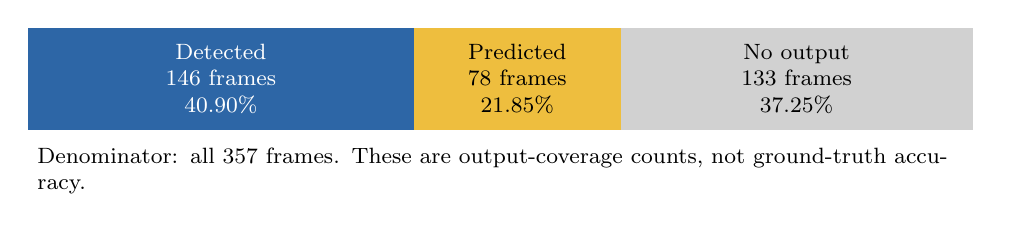
\begin{tikzpicture}[x=1cm,y=1cm,font=\footnotesize]
 \fill[observedBlue] (0,0) rectangle (4.907563,1.3);
 \fill[predictedGold] (4.907563,0) rectangle (7.529412,1.3);
 \fill[black!18] (7.529412,0) rectangle (12,1.3);
 \node[text=white,align=center] at (2.453782,0.65)
   {Detected\\146 frames\\40.90\%};
 \node[align=center] at (6.218488,0.65)
   {Predicted\\78 frames\\21.85\%};
 \node[align=center] at (9.764706,0.65)
   {No output\\133 frames\\37.25\%};
 \node[anchor=north west,text width=12cm,align=left] at (0,-0.1)
   {Denominator: all 357 frames. These are output-coverage counts, not ground-truth accuracy.};
\end{tikzpicture}
\caption{Frame-level coverage of observed, predicted, and missing ball outputs.
Predictions are not counted as model detections.}
\end{figure}

\subsection{Trajectory Fragmentation and Role Stability}

Under the specified break rules, the run produces 60 temporary person IDs
with valid observations, 218 person fragments, and five local ball fragments.
Sixty IDs do not imply sixty real players.
The 218 fragments cannot all be attributed to identity switches: leaving
the region, missing observations, role changes, and conservative break rules
also create fragments.

The shared trajectory manager records 167 breaks associated with missing,
invalid, or duplicate conditions, 41 role-change breaks, and two position-jump
breaks. These counters include person and ball management events; they are
not manually annotated identity switches.
This input contains no repeated same-frame IDs, so that safeguard was not
triggered. Duplicate detections of the same real person under different IDs
may still occur.

This fragmentation means the current records do not support continuous
individual running measurements. V0.7 preserves fragments and exposes the
risk instead of hiding it through cross-ID stitching.

\subsection{Team Observation Time and Position Distributions}

Table~\ref{tab:heat} summarizes accumulated heatmap values.
Team B's higher person-seconds may reflect visible-person counts, occlusion,
detection availability, or team-classification differences.
It cannot be interpreted as possession or tactical superiority.

\begin{table}[htbp]
\centering
\caption{Summary of accepted local team-position samples.}
\label{tab:heat}
\begin{tabular}{lrr}
\toprule
Metric & Team A & Team B\\
\midrule
Accepted person samples & 1,031 & 1,666\\
Cumulative person-seconds & 34.37 & 55.53\\
Time with at least one accepted member (s) & 10.53 & 11.87\\
Maximum cell accumulation (person-s) & 2.57 & 2.40\\
\bottomrule
\end{tabular}
\end{table}

\begin{figure}[htbp]
\centering
\PitchHeatPanel{Team A}{\TeamAHeatCells}
\hspace{1.2cm}
\PitchHeatPanel{Team B}{\TeamBHeatCells}
\par\smallskip
{\small
\textcolor{heatLow}{Low}\quad
\textcolor{heatMid}{Medium}\quad
\textcolor{heatHigh}{High}\qquad
Shared range: 0--2.57 person-s per nominal $1\,\mathrm{m}^2$ cell.}
\caption{Local position heatmaps redrawn from accepted V0.6 CSV samples.
The panels share a scale and include assigned goalkeepers.
Vector cells preserve the accumulated data without external images.
The paper uses its own color palette and need not match the OpenCV PNG
pixel-for-pixel. Blank space outside the penalty area is outside the analysis
scope, not evidence of no player activity.}
\label{fig:heat}
\end{figure}

\section{Engineering Verification and Reproducibility}

\subsection{Software Tests and Video Verification}

During the original report's verification, all 80 automated tests passed.
They cover detection labels, threshold branches, grass support, role cropping
and voting, ball confirmation and prediction, degenerate homographies,
CSV time alignment, trajectory breaks, heatmap units, and actual synthetic-video
output. Software tests verify program contracts and boundary behavior;
they do not replace recognition-accuracy evaluation on real football footage.

The trajectory output is an H.264 MP4 at $1800\times588$, 30 FPS, 357 frames,
and 11.9 seconds. Full decoding succeeded, and the right-side 2D panel changed
across frames. V0.6 default rendering was also compared with the committed
version at local frames 0, 60, 180, and 356. Pixel-identical results at those
samples show that the shared rendering extensions did not alter the sampled
default V0.6 outputs.

\subsection{Output Protection and Provenance}

Default mode protects existing V0.7 outputs.
Publication uses atomic no-clobber links so that a same-name file created by
another process during encoding is not silently overwritten.
Explicit replacement retains recovery copies of old outputs; if a partial
replacement fails, the files replaced by this invocation are restored.
Directory targets and output symlinks are rejected.
If restoration itself fails, recovery files are retained and the error reports
their locations. This is not a power-loss-proof multi-file transaction.

The report records SHA-256 hashes for the clip, calibration, mapping CSV,
and upstream report. Hashes help identify which files were analyzed; they
do not certify correct detections or physically accurate coordinates.
The V0.6 upstream report does not hash its output CSV, so that upstream report
alone cannot prove the CSV was never edited.

\subsection{Boundaries of the Evaluation}

The report distinguishes three classes of evidence:
\begin{enumerate}
  \item \textbf{Engineering evidence:} passing tests, successful file generation,
        and consistent frame counts and timelines;
  \item \textbf{Output descriptions:} detection rows, mapped rows, state proportions,
        and trajectory fragments;
  \item \textbf{Recognition or physical accuracy:} evidence requiring human labels
        or measured reference data, which is not yet available.
\end{enumerate}
The first two cannot substitute for the third.
Future evaluation should annotate matching inputs and frames under fixed
settings, assess detections and predictions separately, and validate mapping
error using independent geometric references.

\section{Limitations, Footage, and Privacy}

\subsection{Main Limitations}

\begin{enumerate}
  \item \textbf{General-purpose detection:} distant balls occupy few pixels;
        compression, motion blur, occlusion, and white markings can cause
        missed or false detections.
  \item \textbf{Temporary identity:} IDs can fragment or switch between nearby
        people. A small-displacement identity switch may not trigger the
        position-jump safeguard.
  \item \textbf{Match-specific colors:} classification depends on the current
        configuration. Generalization to other matches, lighting conditions,
        and similar referee or goalkeeper kits has not been validated.
  \item \textbf{Restricted geometry:} dimensions are assumed and calibration
        or interpolation can drift. Automatic shot-cut detection, pitch-line
        tracking, and full-match calibration are not implemented.
  \item \textbf{Airborne balls:} ball centers need not lie on the ground plane.
        The 2D point is a projection estimate, not a true ground position,
        ball-speed estimate, or 3D trajectory.
  \item \textbf{Sample size and labels:} development and inspection use one
        highlight video and one short geometric-analysis clip.
        No independent annotated dataset supports broad performance claims.
\end{enumerate}

\subsection{Footage and Public Records}

Because source and redistribution permission have not been verified,
the report neither embeds nor redistributes original match frames and does
not claim ownership of the footage.
Its heatmaps are redrawn from project numerical records solely to document
this engineering run.
Public repository materials focus on code, configuration, documentation,
and tests. Footage, weights, generated outputs, and local editor configuration
remain local. The report contains no personal email address, secret, or private
absolute directory.

\section{Conclusion and Future Work}

The project completes an operational prototype from basic object detection
to restricted spatial visualization.
The V0.1--V0.7 iterations connect each change to a concrete problem and
progressively establish annotated video, CSV records, 2D mapping, short
trajectories, position heatmaps, and a quality summary.
For independent learning and portfolio demonstration, the prototype stage
can be considered complete.

Completion does not imply full-match analytics capability.
The next priority is not a larger set of statistics, but a small manually
annotated evaluation set, identity-continuity inspection, independent
ground-plane references, and longer continuous footage with fewer cuts.
Physical running distance, speed, or tactical quantitative analysis should
only be attempted after the relevant errors have been validated.

\appendix
\section{Project Structure and Reproduction Commands}

\begin{lstlisting}
Soccer-Video-Analysis/
  README.md
  requirements.txt
  src/
    detect.py
    team_classifier.py
    ball_tracker.py
    homography.py
    pitch.py
    map_pitch.py
    calibrate.py
    analytics.py
  config/
    v06_pitch_calibration.json
  tests/
  docs/
    versions/
    paper/
      soccer_project_report.tex
      soccer_project_report_en.tex
  data/
  outputs/
\end{lstlisting}

\noindent\textbf{Environment and detection stage:}
\begin{lstlisting}[language=bash]
python3 -m venv .venv
source .venv/bin/activate
pip install -r requirements.txt

ffmpeg -n -i data/soccervideo.mp4 \
  -vf "fps=30" -c:v libx264 -pix_fmt yuv420p -an \
  data/soccervideo_cfr.mp4

python src/detect.py
\end{lstlisting}
Run the conversion only when the corresponding input exists and the CFR output
has not already been generated. Existing footage must not be overwritten.
Model weights may need to be downloaded on first use.

\noindent\textbf{Continuous clip, local mapping, and analytics:}
\begin{lstlisting}[language=bash]
ffmpeg -n -i data/soccervideo_cfr.mp4 \
  -vf "trim=start_frame=2241:end_frame=2598,setpts=PTS-STARTPTS" \
  -an -c:v libx264 -pix_fmt yuv420p -movflags +faststart \
  data/v06_homography_clip.mp4

python src/map_pitch.py
python src/calibrate.py --review
python src/analytics.py
python -m unittest discover -s tests
\end{lstlisting}

\noindent\textbf{Alternative visualization settings without replacing defaults:}
\begin{lstlisting}[language=bash]
python src/analytics.py \
  --trail-seconds 2 \
  --max-person-step-m 1.5 \
  --max-ball-step-m 5 \
  --output-dir outputs/v07_alternative
\end{lstlisting}

\section{Current Key Parameters}

\small
\begin{longtable}{@{}p{5.3cm}p{2.1cm}p{7.6cm}@{}}
\caption{Current default settings and their interpretation.}\\
\toprule
Parameter & Value & Interpretation\\
\midrule
\endfirsthead
\toprule
Parameter & Value & Interpretation\\
\midrule
\endhead
Model input size & 960 & Ultralytics \code{imgsz}; not the source resolution\\
Person display threshold & 0.5 & Controls displayed person detections\\
Person tracking input threshold & 0.1 & Retains weaker association evidence\\
Ball candidate threshold & 0.18 & Small-object candidate score, not ball accuracy\\
Minimum grass support & 0.25 & Anchor-neighborhood color heuristic\\
Ball confirmation hits & 2 & Additional applicable evidence is still required\\
Maximum ball prediction gap & 8 frames & Approximately 0.27 s at 30 FPS\\
Base ball association distance & 120 pixels & Image-space gate, expanded with missing frames\\
Maximum ball-box side & 48 pixels & Shape filtering\\
Ball aspect-ratio range & 0.35--1.8 & Not a physical sphericity constraint\\
Ball grayscale standard deviation & 25 & One appearance-evidence threshold\\
Ball saturation threshold & 180 & Alternative to texture evidence\\
Old-velocity smoothing weight & 0.65 & Independent image-space ball smoothing\\
Nominal pitch size & $105\times68$ m & Not surveyed or a metric-accuracy guarantee\\
Manual keyframes & 13 & Calibration within one continuous shot\\
Maximum calibration fit residual & 12 pixels & Rejection threshold on fitted-point RMSE\\
Displayed trajectory history & 2 s & Recent history in the current contiguous fragment\\
Person jump threshold & 1.5 nominal m/frame & Visualization guard only\\
Ball jump threshold & 5 nominal m/frame & Not a true-speed measurement\\
Heatmap cell size & $1\times1$ nominal m & Accumulated person-seconds\\
\bottomrule
\end{longtable}
\normalsize

\section{Calibration Keyframes and Fit Residuals}

\begin{table}[htbp]
\centering
\caption{Manual calibration snapshot. Fit residuals are not independent
geometric accuracy measurements.}
\small
\begin{tabular}{rrrr}
\toprule
Local frame & Local time (s) & Reference points & Fit RMSE (pixels)\\
\midrule
0   & 0.00  & 6 & 3.34\\
30  & 1.00  & 7 & 3.33\\
60  & 2.00  & 7 & 4.67\\
90  & 3.00  & 6 & 2.05\\
120 & 4.00  & 7 & 5.64\\
150 & 5.00  & 6 & 4.73\\
180 & 6.00  & 6 & 3.18\\
210 & 7.00  & 6 & 7.41\\
240 & 8.00  & 6 & 4.11\\
270 & 9.00  & 5 & 1.65\\
300 & 10.00 & 5 & 2.83\\
330 & 11.00 & 5 & 1.63\\
356 & 11.87 & 5 & 2.83\\
\bottomrule
\end{tabular}
\end{table}

\section{CSV Fields, Artifacts, and Archive Snapshot}

The core V0.5 fields are:
\begin{lstlisting}
frame,time,track_id,role,x1,y1,x2,y2,confidence,ball_state
\end{lstlisting}
V0.6 adds source frame and time, shot ID, anchor coordinates, pitch coordinates,
mapping validity, reason, and position basis.
V0.7 JSON adds fragment summaries, per-frame counts, ball coverage, exclusions,
settings, hashes, and limitations.
Predicted balls have empty \code{confidence}, and all balls have empty
\code{track_id}.

\begin{table}[htbp]
\centering
\caption{Principal final artifacts retained locally.}
\small
\begin{tabularx}{\linewidth}{@{}LL@{}}
\toprule
Relative path & Contents\\
\midrule
\path{outputs/v05_ball_tracking.mp4} & Full-footage detection, roles, and ball association\\
\path{outputs/v05_detections.csv} & Upstream person and ball records\\
\path{outputs/v06_pitch_mapping.mp4} & Local clip and 2D positions\\
\path{outputs/v06_pitch_mapping.csv} & Valid and invalid mapping records\\
\path{outputs/v06_pitch_mapping.json} & Upstream provenance and calibration information\\
\path{outputs/v06_calibration_review.jpg} & Landmark and projected pitch-line inspection\\
\path{outputs/v07_local_trajectories.mp4} & Short contiguous 2D trajectories\\
\path{outputs/v07_team_heatmaps.png} & Shared-scale team position distributions\\
\path{outputs/v07_summary.json} & Statistics, exclusions, settings, and provenance hashes\\
\bottomrule
\end{tabularx}
\end{table}

The report describes the V0.7 local working-tree and output snapshot recorded
on October 3, 2026.
At that snapshot, the last known remote commit was V0.6 commit \code{1b57822}.
V0.7 and the report were not automatically committed or uploaded during
that preparation. The repository link is a code entry point, not evidence
that every local artifact has been published.
This English edition translates the recorded snapshot rather than claiming
a new experimental run.

\noindent\textbf{Input SHA-256 snapshot:}
\begin{lstlisting}
clip:
81094b249c550c15fdc8e017fab4870cb04932d3706eeddfbf951dff585a6c38
calibration:
995f5fb76dad7436569f5bbed7d9910a71ae3b4d15153e3bee87c249eb80436b
mapping_csv:
995e54fd82b551d2c91621d5d29b6c5b0e1f12634411adebf54810112add307e
mapping_report:
6ec7db7b80a208a0746886efbae5fcc05b35b01ef1343f1af9be2ec08cad6eb3
\end{lstlisting}

\section*{Writing and Archival Note}
\addcontentsline{toc}{section}{Writing and Archival Note}
This report was compiled from project code, version READMEs, and local CSV/JSON
outputs. AI assistance was used in preparing the LaTeX draft and the English
edition. It is an independent engineering archive, not a published or
peer-reviewed paper. All statistics must be interpreted according to their
record semantics. Further claims about recognition accuracy, real-player
identity, or physical motion require additional validation.

\begin{thebibliography}{9}
\addcontentsline{toc}{section}{References}

\bibitem{yolo11}
Ultralytics.
\emph{Ultralytics YOLO11: Official Model Documentation}.
\url{https://docs.ultralytics.com/models/yolo11/}.
Accessed October 3, 2026.

\bibitem{bytetrack}
Yifu Zhang, Peize Sun, Yi Jiang, et al.
\emph{ByteTrack: Multi-Object Tracking by Associating Every Detection Box}.
arXiv:2110.06864, 2021.
\url{https://arxiv.org/abs/2110.06864}.

\bibitem{opencv}
OpenCV.
\emph{Basic Concepts of the Homography Explained with Code}.
\url{https://docs.opencv.org/4.x/d9/dab/tutorial_homography.html}.
Accessed October 3, 2026.

\bibitem{ffmpeg}
FFmpeg.
\emph{FFmpeg Filters Documentation}.
\url{https://ffmpeg.org/ffmpeg-filters.html}.
Accessed October 3, 2026.

\bibitem{project}
JIAHE35.
\emph{Soccer-Video-Analysis: Project Code and Version Documentation}.
\url{https://github.com/JIAHE35/Soccer-Video-Analysis}.
Measured values in this report refer to the local V0.7 output snapshot.

\end{thebibliography}
\end{document}
